\section{Other Nonlinear Methods}

\subsection{KNN Classification}

\begin{center}
	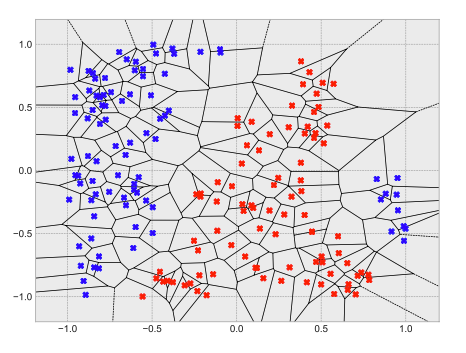
\includegraphics[width=0.6\columnwidth]{knn.png}
\end{center}

This method does not need any training and classification is done during test time. For a given training set $D$ it works as follows:
\begin{enumerate}
	\item Pick $k$ and distance metric $d$
	\item For given $x$, find among $x_1,...,x_n \in D$ the $k$ closest to $x \to x_{i_1},..., x_{i_k}$
	\item Output the majority vote of labels $y_{i_1},..., y_{i_k}$
\end{enumerate}

This method is very sensitive to $k$ and becomes unstable in high dimensions. We might need large $n$ for good results but computation can be reduces when allowing for some error probability.

\subsection{Decision Trees}

\begin{center}
	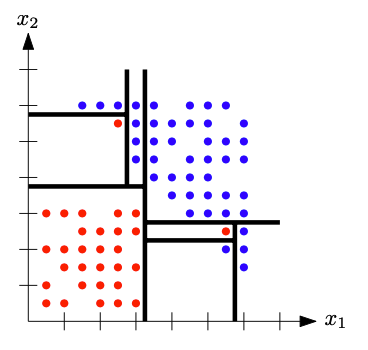
\includegraphics[width=0.52\columnwidth]{decision-tree}
\end{center}

A decision tree returns a partition of $X$ with sets aligned with the main axis. A given $x$ is assigned the majority class of the partition it lands in. The partitions can be modelled as leaf nodes of a binary tree. Single trees can easily overfit to noise, we have to choose the depth of the tree carefully.